Per evidenziare eventuali tendenze degli attributi, è stata effettuata 
un'analisi descrittiva sui dati integrati.

Come si può osservare in Figura~\ref{fig:weather-stations}, abbiamo mostrato su 
una mappa la posizione delle stazioni meteorologiche e delle trappole per 
zanzare. 

\begin{figure}[htb]
	\centering
	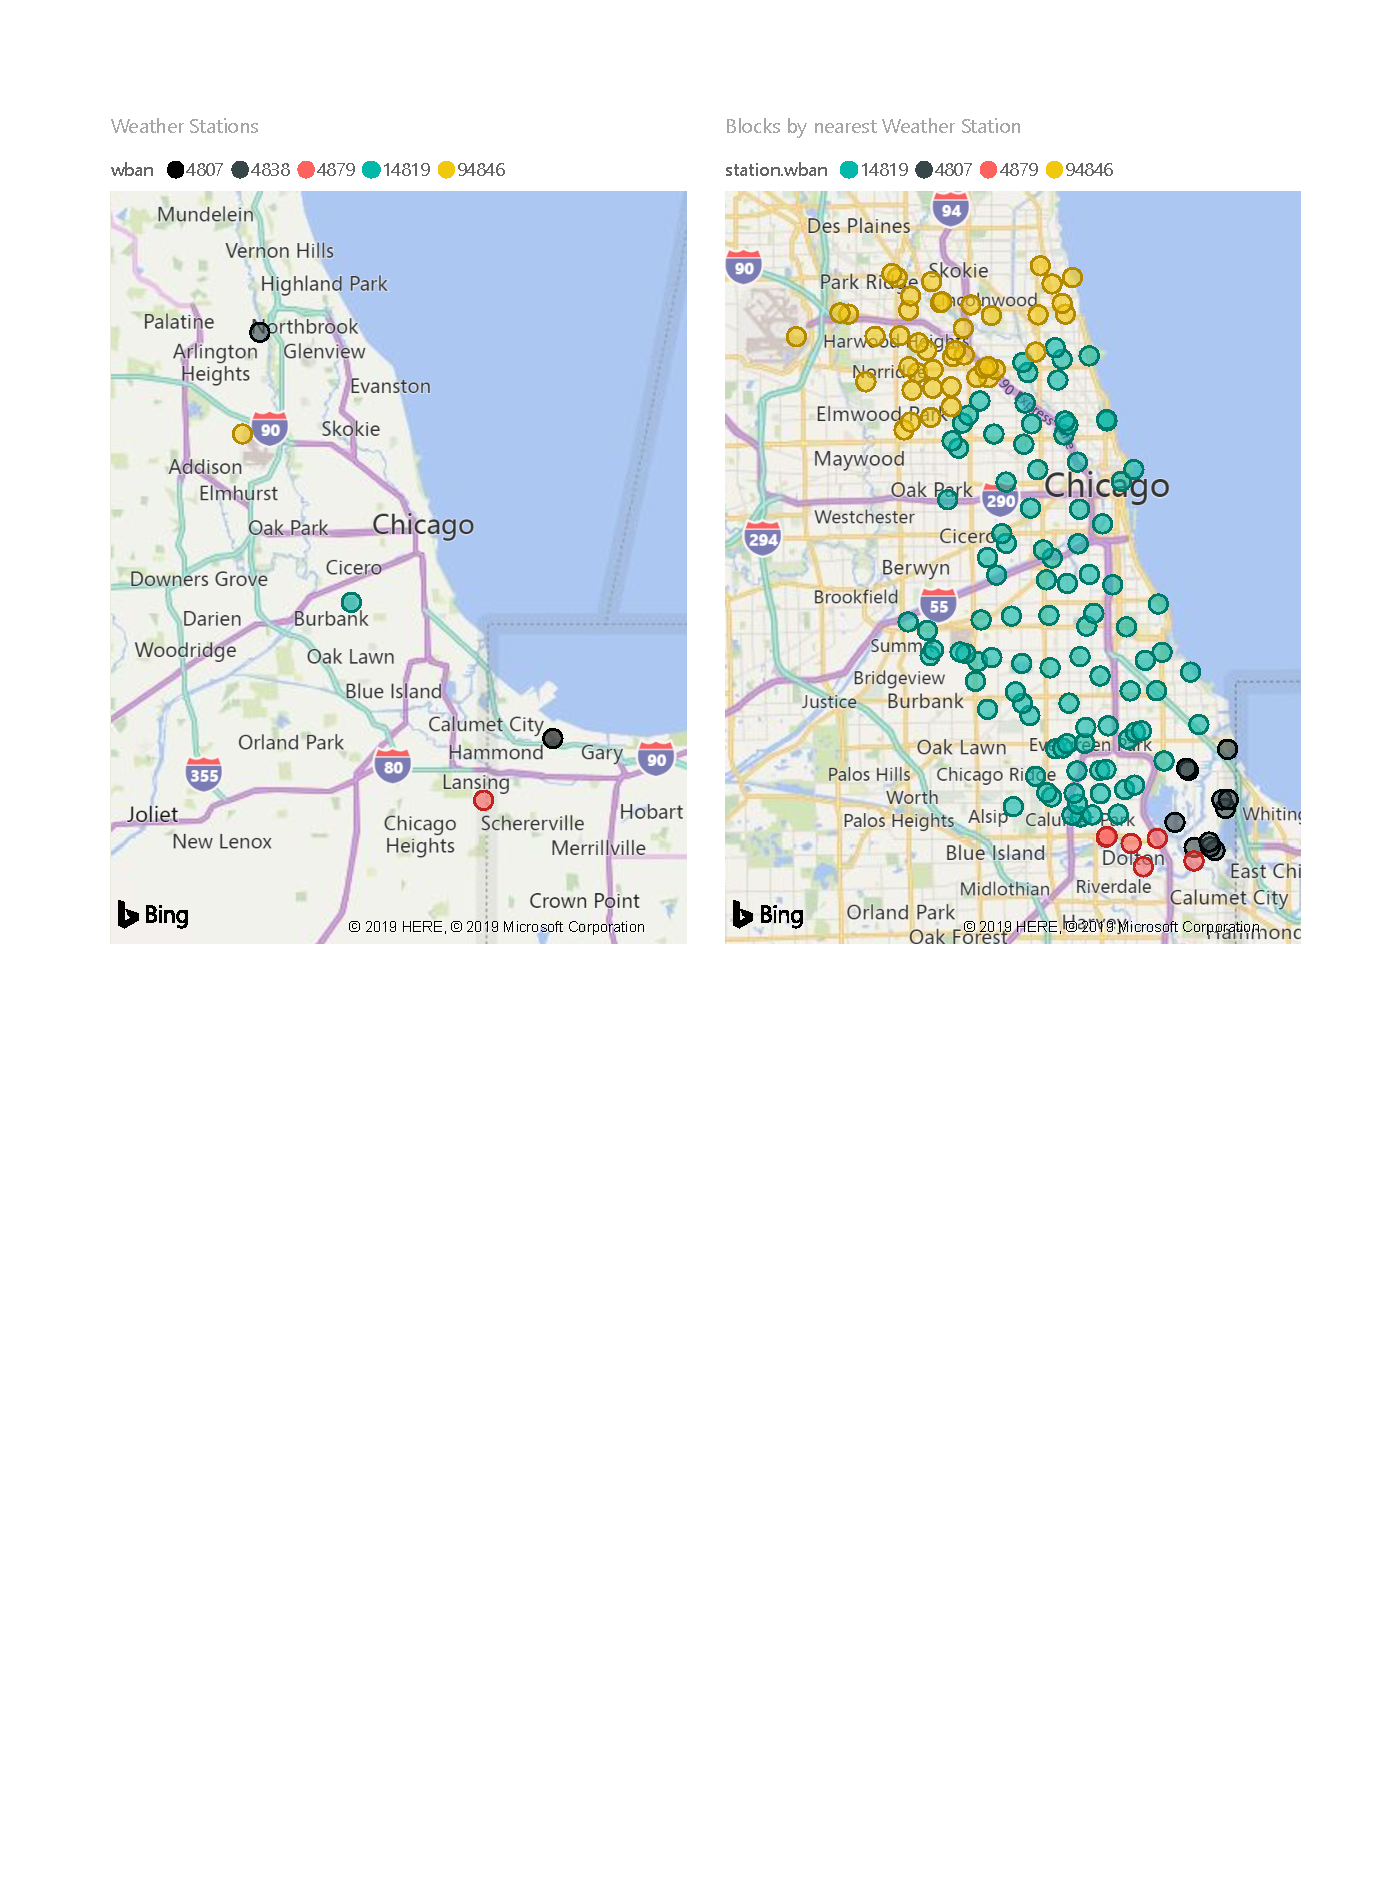
\includegraphics[width=0.4\columnwidth]{images/WeatherStations}
	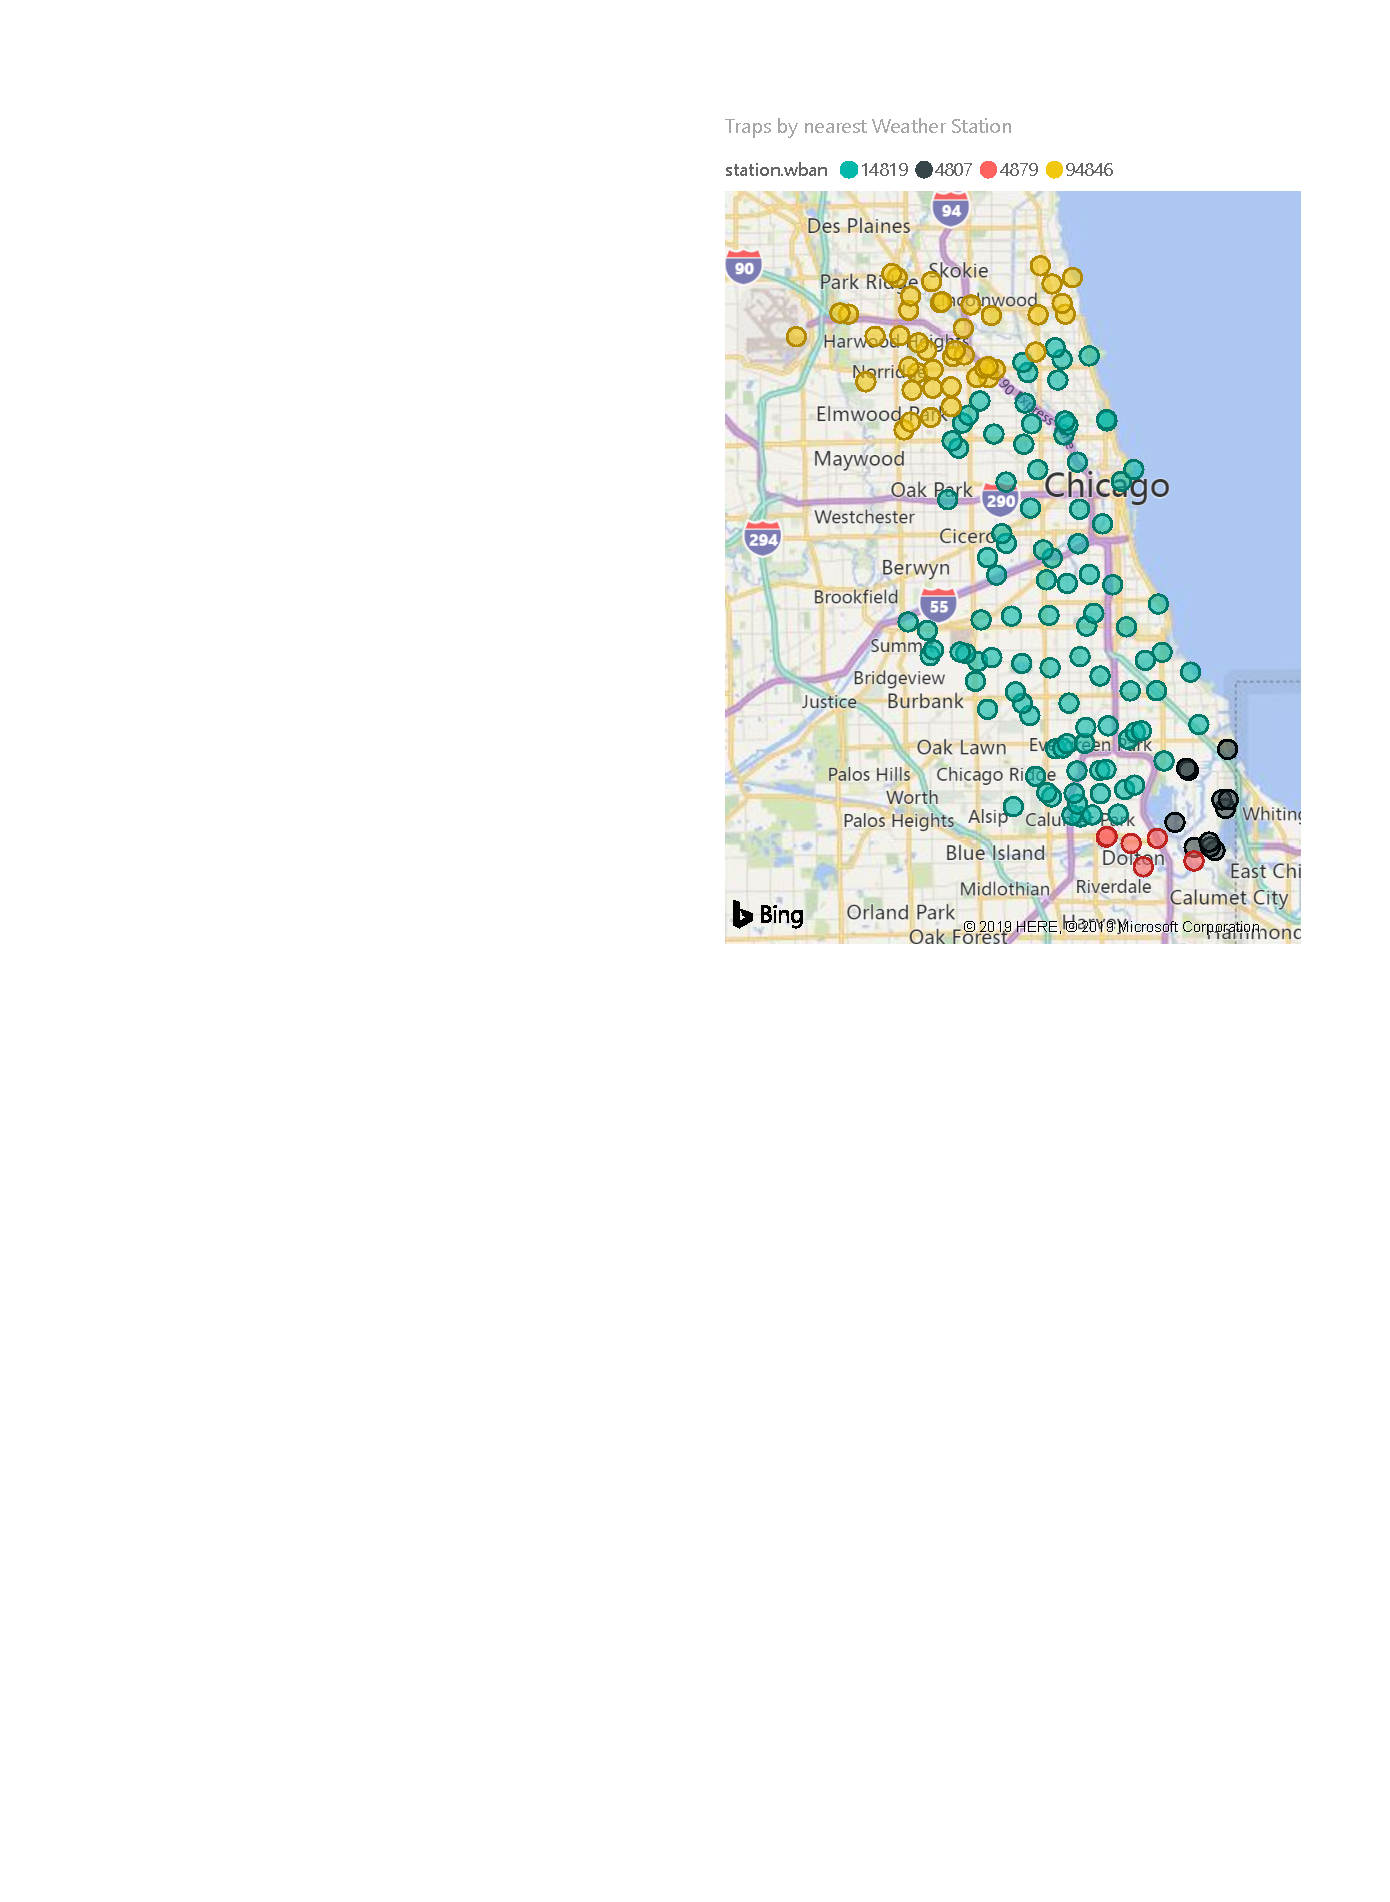
\includegraphics[width=0.4\columnwidth]{images/TrapsByNN}
	\caption{Mappe delle stazioni meteorologiche e delle trappole per zanzare 
	classificate in base alla stazione meteo più vicina}
	\label{fig:weather-stations}
\end{figure}

Alcune osservazioni che emergono dall'analisi dei dati sono elencate di 
seguito, ulteriori visualizzazioni sono inoltre mostrate nel 
Capitolo~\ref{chap:analisi-training} della Parte III.
\begin{itemize}
	\item il 92\% dei test ha un risultato negativo;
	\item il 95\% delle trappole è di tipo Gravid;
	\item i test vengono effettuati solamente nei giorni lavorativi, in 
	particolare tra il giovedì e il venerdì;
	\item il 66\% delle trappole ottiene i dati meteo dalla stazione Chicago 
	Midway International Airport (WBAN 14819);
	\item nessuna trappola ottiene i dati meteo dalla stazione Palwaukee 
	Municipal Airport (WBAN 4838);
	\item un piccolo numero di trappole avrebbe potuto ottenere i dati meteo 
	dalle stazioni Gary/Chicago Airport (WBAN 4807) e Lansing Municipal Airport 
	(WBAN 4879), se questi fossero stati disponibili per l'intero arco 
	temporale;
	\item la media dei valori assunti dalle colonne \texttt{is\_suspicious} è 
	0,017, valore molto buono poiché prossimo allo 0;
	\item mediamente vengono catturate 13 zanzare in ogni test.
\end{itemize} 
